\section{Gegevensmodel}
\subsection{NMEA}
NMEA is een standaardprotocol voor het
weergeven van GPS-data. Dit ziet er zo uit: \\
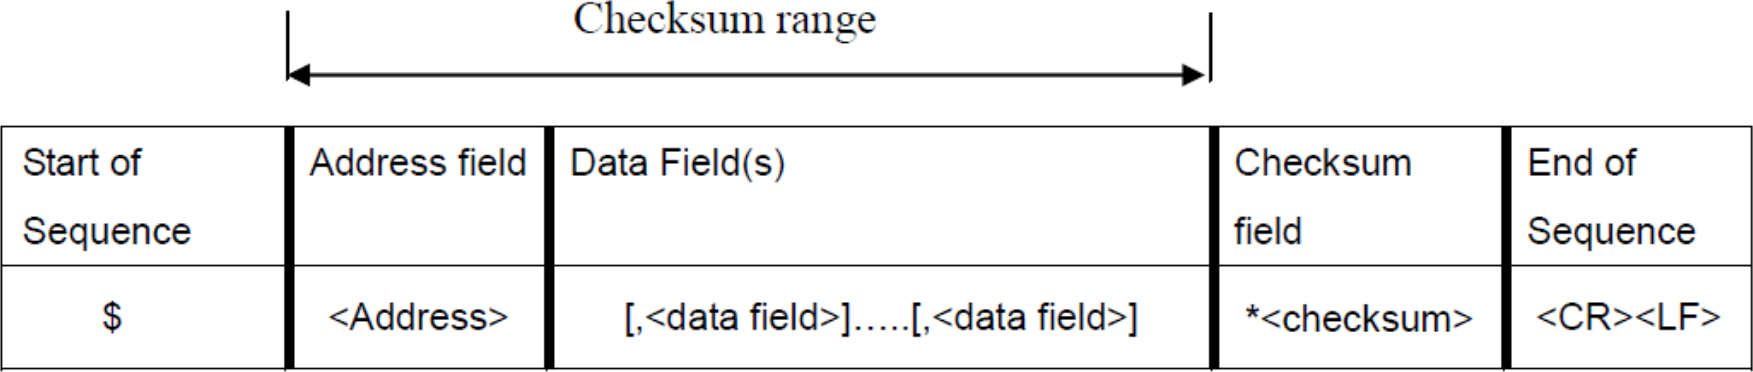
\includegraphics[width=\textwidth]{technical/nmea}
\\Hierbij is het adres veld in het formaat ``aaccc'', waarbij ``aa'' het
Talker ID is en ``ccc'' het soort bericht. Velden zijn gesepareerd met
een ``,''.
\citep{Navspark}\\\\
Het belangrijkste deel van dit format zijn de GNS-berichten
(GNSS-data). Deze berichten zien er als volgt uit:\\
\texttt{\$GPGNS,091547.00,5114.50897,N,00012.28663,W,AA,10,0.83,111.1,45.6,,,V*71}

\begin{tabularx}{\textwidth}{| l | l | l | l | X |}
    \hline
    \textbf{Veld} & \textbf{Naam} & \textbf{Formaat} & \textbf{Voorbeeld} & \textbf{Beschrijving}          \\ \hline
    0             & xxGNS         & string           & \$GPGNS            & GNS ID (xx = current Talker)   \\ \hline
    1             & Tijd          & hhmmss.ss        & 091547.00          & Tijd (UTC)                     \\ \hline
    2             & Latitude      & ddmm.mmmmm       & 5114.50897         & Latitude (graden en minuten)   \\ \hline
    3             & NS            & character        & N                  & Noord/Zuid                     \\ \hline
    4             & Longtitude    & dddmm.mmmmm      & 00012.28663        & Longtitude (graden en minuten) \\ \hline
    5             & EW            & character        & E                  & Oost/West                      \\ \hline
    6             & posMode       & character        & AA                 & Positionering mode             \\ \hline
    7             & numSV         & numeric          & 10                 & Aantal satellieten             \\ \hline
    8             & HDOP          & numeric          & 0.83               & Horizontal dilution precision  \\ \hline
    9             & alt           & numeric          & 111.1              & Hoogte boven zeeniveau         \\ \hline
    10            & sep           & numeric          & 45.6               & Geoïde separatie               \\ \hline
    11            & diffAge       & numeric          & -                  & Leeftijd correctie             \\ \hline
    12            & diffStation   & numeric          & -                  & ID GPS-correctie station       \\ \hline
    13            & navStatus     & character        & V                  & Navigatie Status               \\ \hline
    14            & cs            & hexadecimal      & *71                & Checksum                       \\ \hline
    15            & <CR><LF>      & character        & -                  & Carriage Return                \\ \hline
\end{tabularx}
\citep[p. 116]{UBlox8}\\

De uiteindelijke data die we gaan gebruiken is:
ID, Tijd (UTC), Latitude, en Longtitude.

\newpage
\subsection{UBX}
Om DGPS-data binnen te krijgen is het UBX-protocol noodzakelijk. Met UBX is het
mogelijk de ruwe data binnen te krijgen en op te slaan.

Deze ruwe data wordt door de ontvanger aangeleverd in een Ublox binary formaat.
Deze data is dan nog niet te gebruiken om correcties te doen. Eerst moet de data
geconverteerd worden naar RINEX (Receiver Independent Exchange Format). Dit kan
gedaan worden met een programma genaamd convbin.
De informatie die hieruit komt ziet er ongeveer als volgt uit:

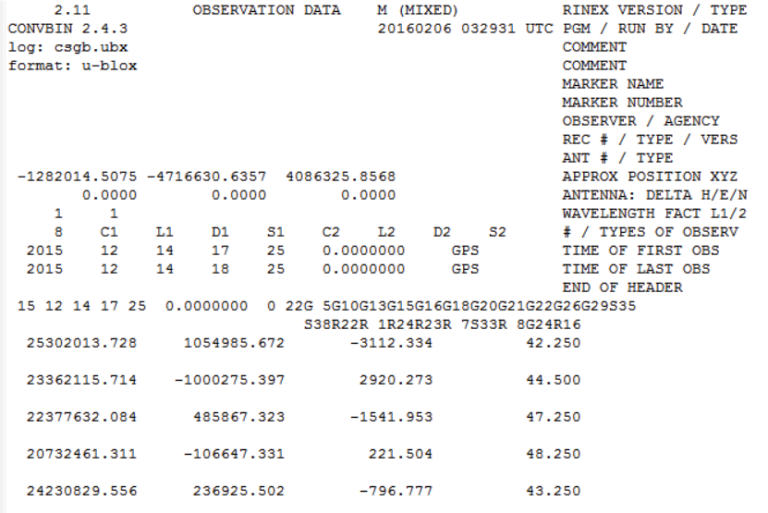
\includegraphics[width=\textwidth]{technical/obsfile}
\citep{rtklibexplorer}\\

Deze informatie kan geïnterpreteerd worden, door een bibliotheek zoals RTKLIB.

Verder wordt UBX gebruikt om instellingen op de ontvanger te doen.

Om UBX-berichten te kunnen versturen moeten deze op een bepaalde manier zijn
opgesteld. Dit ziet er als volgt uit:\\
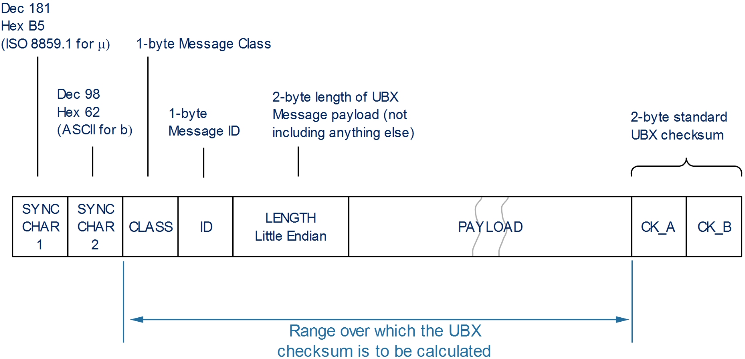
\includegraphics[width=\textwidth]{technical/ubx}
\citep[p. 132]{UBlox8}\\

Eerst worden er 2 synchronisatie karakters verstuurd, 0xB5 0x62. Dit is bij
alle UBX-berichten hetzelfde. Vervolgens wordt het klasse id van het bericht
verstuurd en het bericht id. Dit is zodat de ontvanger weet met wat voor bericht
het te maken heeft. Dan wordt de lengte van het bericht verstuurd. Dit wordt
gedaan in little endian. Vervolgens wordt de payload, het bericht zelf
verstuurd. Als laatste wordt een checksum verstuurd. De checksum wordt berekend
vanaf het klasse id tot aan de checksum zelf.

Een belangrijk onderdeel van het instelling van de ontvanger dat wij gaan
gebruiken is het instellen van de berichten die we binnen krijgen.
Dat wordt als volgt gedaan:
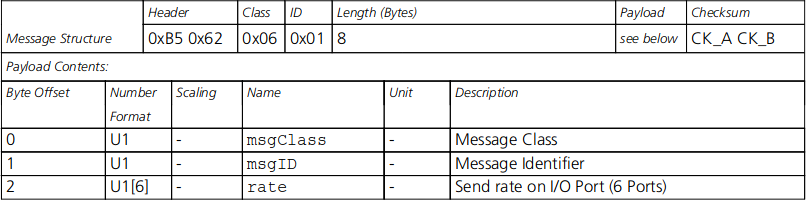
\includegraphics[width=\textwidth]{technical/set-rate}
\citep[p. 171]{UBlox8}\\

De eerste 2 bytes van de payload bestaan uit het klasse id en het bericht id van
het bericht dat ingesteld moet worden. Vervolgens wordt de rate verstuurd. De
rate is in dit geval per hoeveel keer de ontvanger GPS-data ontvangt de
ontvanger het ook moet versturen.
Hierbij is het eerste byte voor I2C, het tweede byte voor UART, het derde byte
voor USB en het vierde byte voor SPI. De rest is gereserveerd.
\citep[p. 11]{UBlox8}

Wanneer het bericht goed verzonden is wordt hierop door de receiver een
acknowledge verstuurd. Deze moet ontvangen worden voordat de receiver weer
kan verzenden.

\subsection{Data routing}
De Smart Markers versturen hun data naar de KPN LoRa portal.

Vanuit deze portal is het mogelijk om via een HTTPS verbinding, welke dus beveiligd is,
te versturen naar een eigen API.

Voor dit project komt het binnen in een PHP script, welke de verkregen data samen met het
moment van ontvangen in een SQL-database zet. Deze database draait op dezelfde server als
de webserver. De meetpunten worden hierbij in de decimale notatie opgeslagen.

Deze server draait bij één van de projectleden thuis. Deze bestaat uit een virtuele
machine met daarop CentOS 7. Deze draait de Apache webserver gecombineerd met een
MariaDB SQL-database.

Het HTTPS certificaat wordt verkregen met een certificaat van Let's Encrypt.org

\subsection{Database}
\label{sec:database}
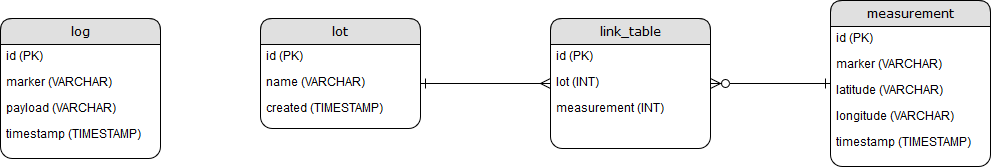
\includegraphics[width=\textwidth]{technical/erd.png}

De log tabel bevat geen relaties met de andere tabellen en is ook niet van
invloed op de werking van het systeem. Deze bestaat enkel voor het makkelijker
debuggen en controleren van de binnengekomen berichten.

Meetpunten worden opgeslagen in de measurement tabel, waarna ze via de webpagina
eventueel toegevoegd kunnen worden aan een perceel. De percelen worden opgeslagen
in de tabel lot.

Omdat dit een veel op veel relatie is, een meetpunt kan meerdere percelen begrenzen en
een perceel heeft meerdere meetpunten, is er een koppeltabel, link\_table, nodig.
Deze koppelt het id van een perceel aan het ID van de bijbehorende meetpunten.
